\chapter{查找}\label{DS07}

\section{关键字与平均查找长度}\label{DS07-definition}

查找表为同类型记录的集合。主关键字唯一标识记录，次关键字可对应多条记录；静态表仅查找，动态表还支持插入、删除。存储为数组或链表不能单独决定静态、动态属性。

\[ASL=\sum_i p_iC_i.\]

先确定事件集合、概率\(p_i\)与代价\(C_i\)。成功事件为已有记录，失败事件可按关键字区间或初始散列地址分布；失败ASL分母未必等于表长或记录数。树结点访问次数、关键字比较次数、外存读盘次数分别统计。

\section{顺序查找与分块查找}\label{DS07-sequential}

无序表逐项比较，等概率成功平均\((n+1)/2\)次，失败比较\(n\)个实际记录。有序递增表从头查找时，当前值等于目标即成功，大于目标才可提前失败。

\par\smallskip\noindent\begin{minipage}{\linewidth}
\begin{codeblock}[language={C++}]
typedef struct {
    ElemType *elem;
    int TableLen;
} SSTable;
int Search_Seq(SSTable ST, ElemType key) {
    ST.elem[0]=key;
    int i;
    for (i=ST.TableLen; ST.elem[i]!=key; --i) ;
    return i;
}
\end{codeblock}
\end{minipage}\par\smallskip

有效记录为\texttt{elem[\allowbreak{}1.\allowbreak{}.\allowbreak{}TableLen]\allowbreak{}}，0号为可写哨兵，空表也需此位置。失败包括哨兵比较时为\(n+1\)次；返回0表示失败。结构体按值传入仍共享指针所指数组，写哨兵会改变原数组0号单元。

静态顺序查找按访问概率非增序排列可减小成功ASL。底稿六记录概率\texttt{0.\allowbreak{}15,\allowbreak{}0.\allowbreak{}05,\allowbreak{}0.\allowbreak{}10,\allowbreak{}0.\allowbreak{}40,\allowbreak{}0.\allowbreak{}28,\allowbreak{}0.\allowbreak{}02}原序ASL为3.67，按概率排序后为2.18。

\textbf{分块查找}要求块间有序、块内可无序，索引记录每块最大关键字及块起始位置。定位第一个最大关键字不小于目标的块，再块内顺序查找。索引折半未遇相等值时，结束的\texttt{low}可指目标块，超过末索引才直接失败。动态更新须维护块范围和索引最大值。

\par\medskip\Needspace{4\baselineskip}\noindent\hypertarget{DS07-E01}{}\label{DS07-E01}\textbf{例 7-1}\par\nobreak\smallskip

查找表有400个元素，查找每个元素的概率相同，采用均匀分块。先顺序查找确定所在块，块内也顺序查找。为使查找效率最高，每块包含元素个数应为（　）。

A. 8　B. 10　C. 20　D. 25

\section{折半查找与判定树}\label{DS07-binary}

折半查找要求\textbf{关键字有序且能随机定位中点}。以下有效范围为\texttt{elem[\allowbreak{}0.\allowbreak{}.\allowbreak{}TableLen-1]\allowbreak{}}，采用闭区间及向下取整中点：

\par\smallskip\noindent\begin{minipage}{\linewidth}
\begin{codeblock}[language={C++}]
int Binary_Search(SSTable L, ElemType key) {
    int low=0, high=L.TableLen-1, mid;
    while (low<=high) {
        mid=(low+high)/2;
        if (L.elem[mid]==key) return mid;
        else if (L.elem[mid]>key) high=mid-1;
        else low=mid+1;
    }
    return -1;
}
\end{codeblock}
\end{minipage}\par\smallskip

循环开始时若目标存在，必在\texttt{[\allowbreak{}low,\allowbreak{}high]\allowbreak{}}；排除相等后用\texttt{mid±1}去掉已比较项，\texttt{low>\allowbreak{}high}表示失败。大下标可用\texttt{low+\allowbreak{}(\allowbreak{}high-low)\allowbreak{}/\allowbreak{}2}防止求和溢出。

判定树成功次数等于内部结点层次，失败次数等于沿途内部结点数。\(n\ge1\)时最大比较次数为\(\lfloor\log_2n\rfloor+1\)。偶数区间取下中点时右子树多一项，树高平衡但未必完全；改取上中点会改变路径。

\par\medskip\Needspace{4\baselineskip}\noindent\hypertarget{DS07-E02}{}\label{DS07-E02}\textbf{例 7-2}\par\nobreak\smallskip

长度为16的顺序表L按关键字有序，采用折半查找，查找一个不存在的元素，关键字比较次数最多为（　）。

A. 4　B. 5　C. 6　D. 7

长度11的表\texttt{7,\allowbreak{}10,\allowbreak{}13,\allowbreak{}16,\allowbreak{}19,\allowbreak{}29,\allowbreak{}32,\allowbreak{}33,\allowbreak{}37,\allowbreak{}41,\allowbreak{}43}中，查33比较\texttt{29,\allowbreak{}37,\allowbreak{}32,\allowbreak{}33}；查12比较\texttt{29,\allowbreak{}13,\allowbreak{}7,\allowbreak{}10}后失败。成功层次分布1、2、4、4个，等概率成功ASL为3；12个失败区间中4个需3次、8个需4次，失败ASL为\(11/3\)。

有序链表缺少常数时间中点访问，折半式比较的对数比较次数无法直接保证对数总访问时间。

\section{二叉搜索树}\label{DS07-bst}

互异关键字BST的左子树全部值小于根、右子树全部值大于根，各子树递归满足。等价判据为中序严格递增。验证可传递全局允许区间；合法值包含整数极值时，用显式边界标志或更宽类型。

\par\smallskip\noindent\begin{minipage}{\linewidth}
\begin{codeblock}[language={C++}]
typedef struct BSTNode {
    int key;
    struct BSTNode *lchild, *rchild;
} BSTNode, *BSTree;
BSTNode *BST_Search(BSTree T, int key) {
    while (T!=NULL && key!=T->key) {
        if (key<T->key) T=T->lchild;
        else T=T->rchild;
    }
    return T;
}
int BST_Insert(BSTree &T, int k) {
    if (T==NULL) {
        T=(BSTree)malloc(sizeof(BSTNode));
        T->key=k;
        T->lchild=T->rchild=NULL;
        return 1;
    } else if (k==T->key) return 0;
    else if (k<T->key) return BST_Insert(T->lchild,k);
    else return BST_Insert(T->rchild,k);
}
void Create_BST(BSTree &T, int str[], int n) {
    T=NULL;
    for (int i=0; i<n; ++i) BST_Insert(T,str[i]);
}
\end{codeblock}
\end{minipage}\par\smallskip

插入默认申请成功，重复关键字返回0；先搜索到空子树才建叶。操作为\(O(h)\)，普通BST最坏可退化到\(O(n)\)；迭代查找工作空间\(O(1)\)。

删除分三类：叶直接断开；单孩子由孩子接替；双孩子用中序前驱或后继替换，再删除原前驱/后继。前驱无右孩子、后继无左孩子，因此归结到前两类。

\par\smallskip\noindent\begin{minipage}{\linewidth}
\begin{codeblock}[language={}]
erase(t,key):
    if t为空: return 空
    if key<t.key: t.lchild=erase(t.lchild,key)
    else if key>t.key: t.rchild=erase(t.rchild,key)
    else:
        if t.lchild为空: 保存t.rchild，释放t，返回保存值
        if t.rchild为空: 保存t.lchild，释放t，返回保存值
        q=t.rchild；沿q.lchild找到右子树最小结点
        t.key=q.key（记录有附加字段时一并复制）
        t.rchild=erase(t.rchild,q.key)
    return t
\end{codeblock}
\end{minipage}\par\smallskip

递归返回删除后的子树根，栈空间\(O(h)\)。复制须带整条记录；要求保留结点身份时采用移接。

\section{AVL插入与删除}\label{DS07-avl}

AVL为任意结点左右高差至多1的BST，平衡因子\(BF=h_L-h_R\)。插入后从新叶向上，找最近失衡祖先\(A\)：

\par\smallskip
{\fontsize{9.3}{12}\selectfont\setlength{\tabcolsep}{2.5pt}\setlength{\LTleft}{0pt}\setlength{\LTright}{0pt}
\begin{longtable}{@{}>{\raggedright\arraybackslash}p{\dimexpr0.37575\linewidth-2\tabcolsep\relax}>{\raggedright\arraybackslash}p{\dimexpr0.62425\linewidth-2\tabcolsep\relax}@{}}
\toprule
失衡路径 & 调整 \\

\midrule\endfirsthead\toprule
失衡路径 & 调整 \\

\midrule\endhead\bottomrule\endfoot
LL & 对A右旋 \\

RR & 对A左旋 \\

LR & 左旋A的左孩子，再右旋A \\

RL & 右旋A的右孩子，再左旋A \\

\end{longtable}}
\par\smallskip

\par\smallskip\noindent\begin{minipage}{\linewidth}
\begin{codeblock}[language={C++}]
void R_Rotate(BSTree &p) {
    BSTNode *lc=p->lchild;
    p->lchild=lc->rchild;
    lc->rchild=p;
    p=lc;
}
void L_Rotate(BSTree &p) {
    BSTNode *rc=p->rchild;
    p->rchild=rc->lchild;
    rc->lchild=p;
    p=rc;
}
\end{codeblock}
\end{minipage}\par\smallskip

引用参数接回新局部根。中间子树按关键字区间转接；若保存高度，先更新下降结点，再更新提升结点。只交换两个根值无法代替链接旋转。

\begin{figure}[H]
\centering
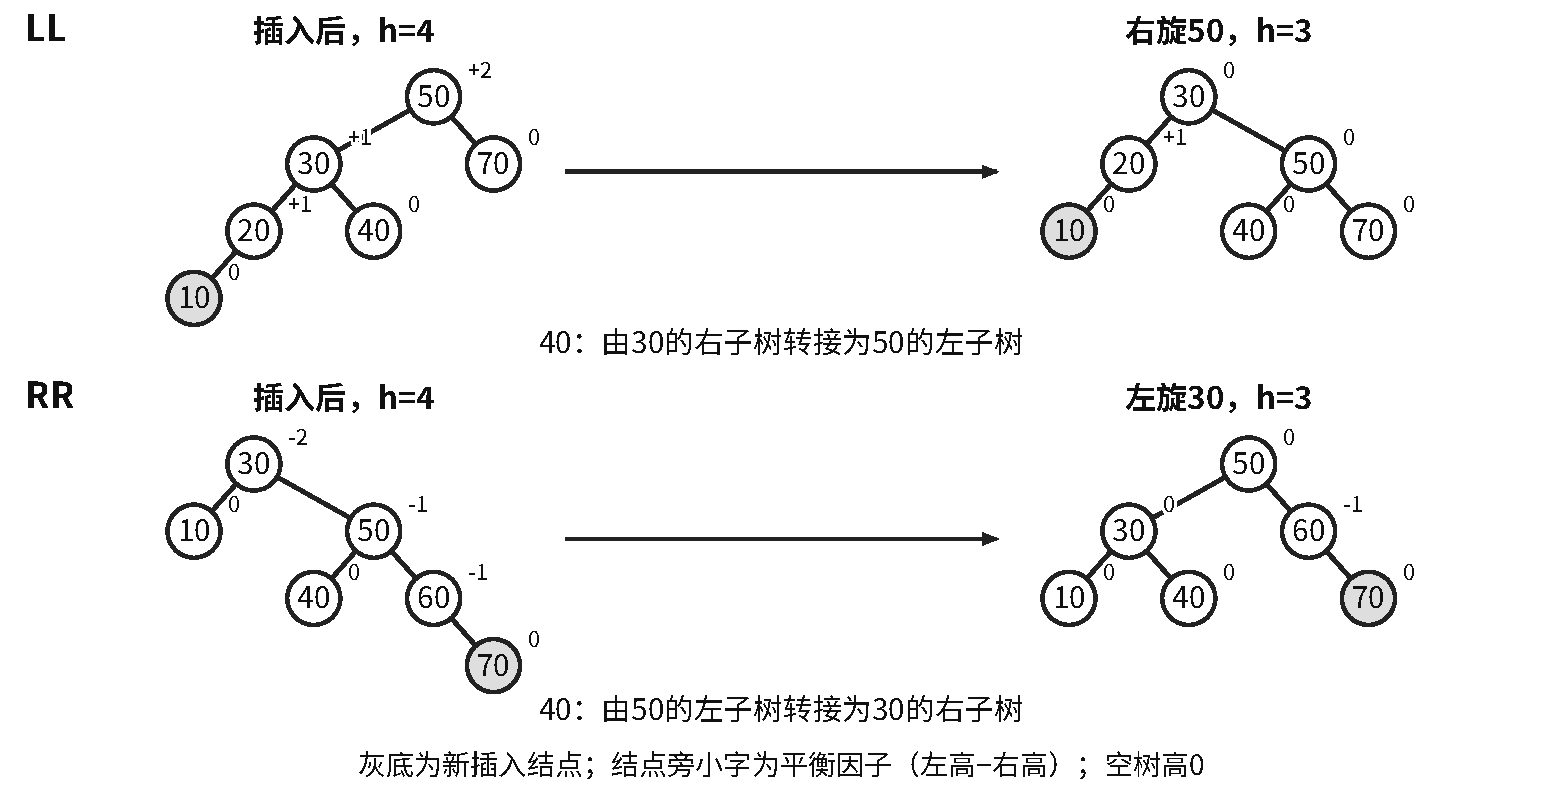
\includegraphics[width=\linewidth,height=108mm,keepaspectratio]{figures/DS_14_avl_rotations.pdf}
\caption{单旋与中间子树}\label{DS07-single-rotation}
\end{figure}

\begin{figure}[H]
\centering
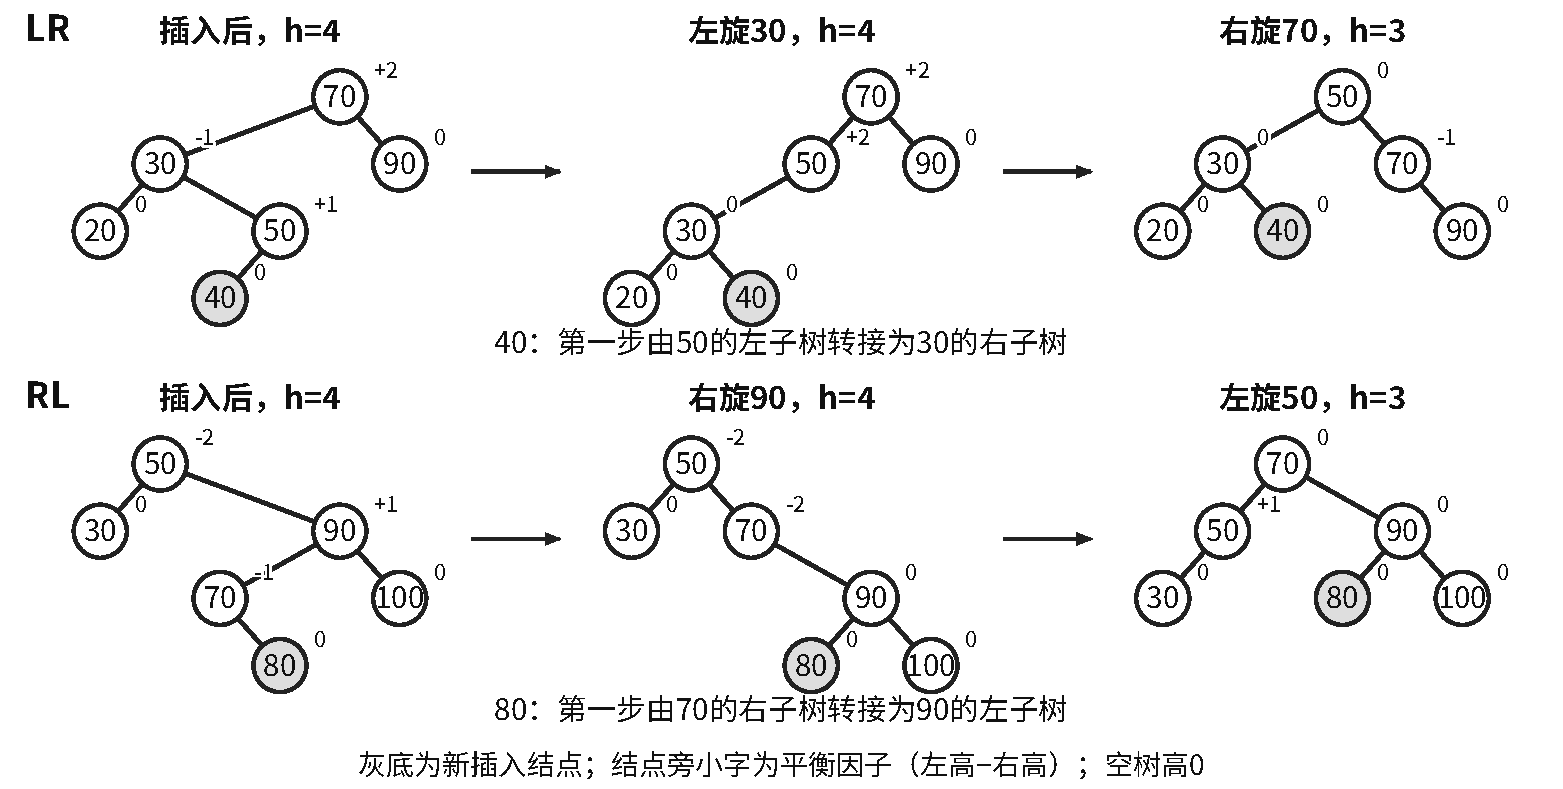
\includegraphics[width=\linewidth,height=108mm,keepaspectratio]{figures/DS_21_avl_double_rotations.pdf}
\caption{双旋的完整两步}\label{DS07-double-rotation}
\end{figure}

\par\medskip\Needspace{4\baselineskip}\noindent\hypertarget{DS07-E03}{}\label{DS07-E03}\textbf{例 7-3}\par\nobreak\smallskip

把34、23、15、98、115、28、107依次插入初始为空的平衡二叉搜索树，要求每次插入后保持AVL性质，给出每步结果。

插入修复最小失衡子树后恢复原高度，可停止向上传播。最少结点数满足\(N(0)=0,N(1)=1\)、\(N(h)=1+N(h-1)+N(h-2)\)，故高\(O(\log n)\)。

\textbf{删除}先按BST删除，再沿实际被移除结点的祖先向上检查；修复后高度仍可能减1，需继续传播。

\par\smallskip
{\fontsize{9.3}{12}\selectfont\setlength{\tabcolsep}{2.5pt}\setlength{\LTleft}{0pt}\setlength{\LTright}{0pt}
\begin{longtable}{@{}>{\raggedright\arraybackslash}p{\dimexpr0.26514\linewidth-2\tabcolsep\relax}>{\raggedright\arraybackslash}p{\dimexpr0.32581\linewidth-2\tabcolsep\relax}>{\raggedright\arraybackslash}p{\dimexpr0.40904\linewidth-2\tabcolsep\relax}@{}}
\toprule
A的BF & 较高孩子的BF & 调整 \\

\midrule\endfirsthead\toprule
A的BF & 较高孩子的BF & 调整 \\

\midrule\endhead\bottomrule\endfoot
\(+2\) & \(+1\)或0 & 右单旋A \\

\(+2\) & \(-1\) & 先左旋孩子，再右旋A \\

\(-2\) & \(-1\)或0 & 左单旋A \\

\(-2\) & \(+1\) & 先右旋孩子，再左旋A \\

\end{longtable}}
\par\smallskip

孩子BF为0时，单旋后高度可保持删除前高度，上层停止受影响。例如\texttt{4(\allowbreak{}2(\allowbreak{}1,\allowbreak{}3)\allowbreak{},\allowbreak{}5)\allowbreak{}}删5后右旋为\texttt{2(\allowbreak{}1,\allowbreak{}4(\allowbreak{}3,\allowbreak{}空)\allowbreak{})\allowbreak{}}，高仍为3。查找、插删最坏均\(O(\log n)\)。

固定高度形态数满足\(C(0)=C(1)=1\)、\(C(h)=C(h-1)^2+2C(h-1)C(h-2)\)，故\(C(2)=3,C(3)=15\)；该量与固定结点数的卡特兰计数不同。

\par\medskip\Needspace{4\baselineskip}\noindent\hypertarget{DS07-E04}{}\label{DS07-E04}\textbf{例 7-4}\par\nobreak\smallskip

一棵无重复关键字的AVL树，中序遍历得到降序序列。正确叙述是（　）。

A. 根的度一定为2　B. 最小元素一定是叶结点

C. 最后插入元素一定是叶结点　D. 最大元素一定没有左子树

\section{红黑树}\label{DS07-redblack}

红黑树为BST并满足：每结点红或黑；根黑；空孩子为黑NIL；红结点的孩子黑；任一结点至后代NIL的路径黑结点数相同。

黑高\(b\)不计当前结点、计终点NIL，NIL自身黑高0。根黑的非空树内部结点数满足

\[2^b-1\le n\le2^{2b}-1.\]

相邻红结点受限，最长路径至多约为最短路径两倍，高度\(O(\log n)\)。

\textbf{插入}先按BST插入红叶：父黑直接结束；父红时看叔。红叔则父叔黑、祖父红并上移；黑叔含NIL，内侧折线先旋父转外侧，再旋祖父并交换提升结点与祖父颜色。最后根黑。旋转次数为常数，变色可能传播到根，完整插入仍\(O(\log n)\)。

\textbf{删除}先化为至多一非空孩子：删红无黑高损失；删黑有红孩子接替时染黑；黑/NIL接替造成缺黑。下表缺黑位置\(x\)为父\(p\)左孩子，兄弟\(w\)在右，近侧为\(w\)左孩子、远侧为\(w\)右孩子：

\par\smallskip
{\fontsize{9.3}{12}\selectfont\setlength{\tabcolsep}{2.5pt}\setlength{\LTleft}{0pt}\setlength{\LTright}{0pt}
\begin{longtable}{@{}>{\raggedright\arraybackslash}p{\dimexpr0.37863\linewidth-2\tabcolsep\relax}>{\raggedright\arraybackslash}p{\dimexpr0.62137\linewidth-2\tabcolsep\relax}@{}}
\toprule
条件 & 修复 \\

\midrule\endfirsthead\toprule
条件 & 修复 \\

\midrule\endhead\bottomrule\endfoot
w红 & w黑、p红，左旋p，重新取兄弟 \\

w黑、双孩子黑 & w红；p红则改黑结束，否则缺黑上移到p \\

w黑、远黑近红 & 近侧黑、w红，右旋w，转为下一行 \\

w黑、远红 & w取p原色、p与远侧黑，左旋p，结束 \\

\end{longtable}}
\par\smallskip

缺黑在右时左右对换；缺黑到根可结束。性质检查同时核对BST、中序、根/NIL、红红相邻及各路径黑高。

\begin{figure}[H]
\centering
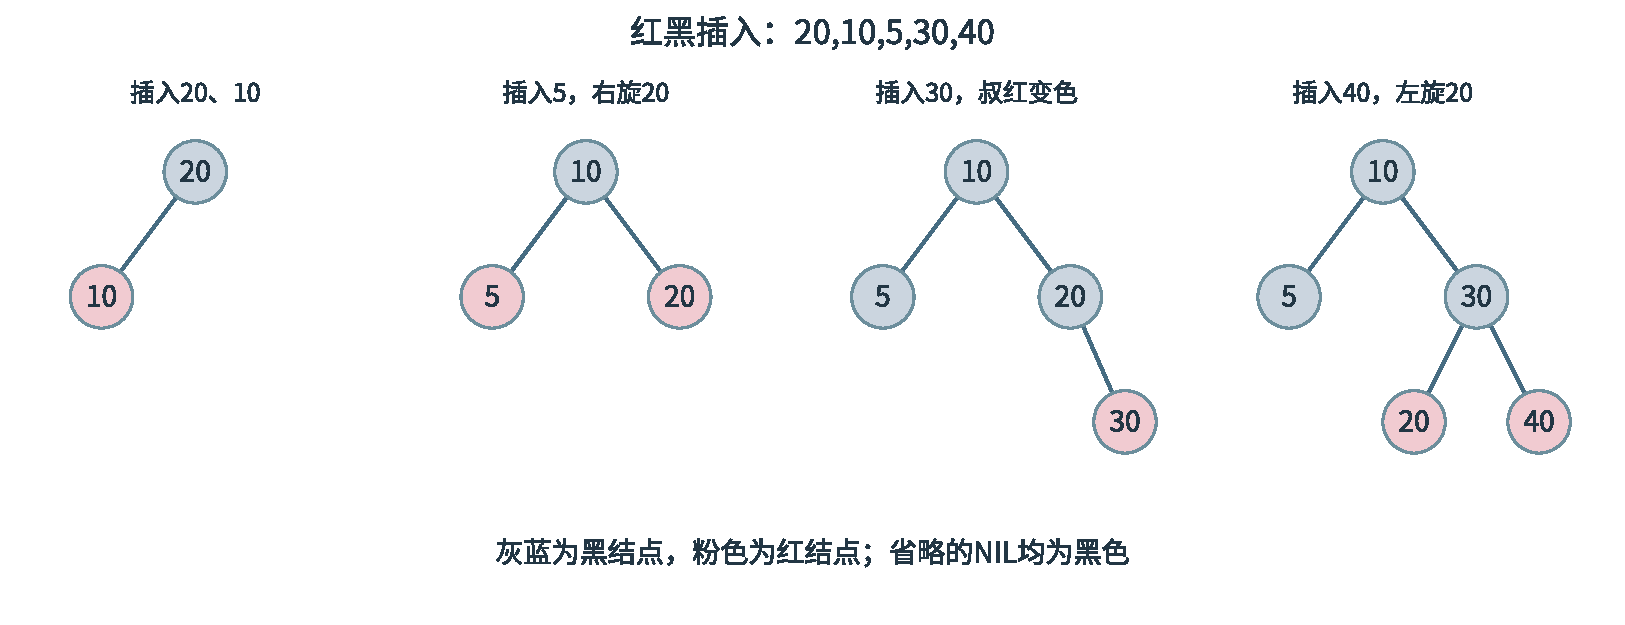
\includegraphics[width=\linewidth,height=108mm,keepaspectratio]{figures/DS07_rb_insert_course.pdf}
\caption{红黑插入的黑叔旋转与红叔变色}\label{DS07-redblack-figure}
\end{figure}

\section{B树的容量、插入与删除}\label{DS07-btree}

\(m\)阶B树每数据结点至多\(m-1\)键、\(m\)孩子；除根外至少\(t-1\)键，\(t=\lceil m/2\rceil\)。非底层数据结点\(k\)键对应\(k+1\)个孩子区间，非叶根至少1键、2孩子；底层数据结点等深。以下\(m\ge3\)，高度\(h\)只计数据层，排除失败空叶。

\[2t^{h-1}-1\le n\le m^h-1.\]

求最大高用最少容量，求最小高用最大容量。外存一结点一页时，查找最多读\(h\)个索引页，结点内部还需关键字比较。

\textbf{插入}沿路径到最底层数据结点插入，溢出则提升中间键、左右分裂，父溢出继续向上。内部分裂同步分配孩子，只有根分裂使高度增加。

\textbf{删除}内部键先以前驱或后继替换，再到底层删除。下溢时优先向有富余的相邻兄弟借：父分隔键下移、兄弟近侧键上移，必要时转接孩子。兄弟无富余则将下溢结点、父分隔键和兄弟合并，父可能继续下溢。空根仅剩一孩子时降层。

\begin{figure}[H]
\centering
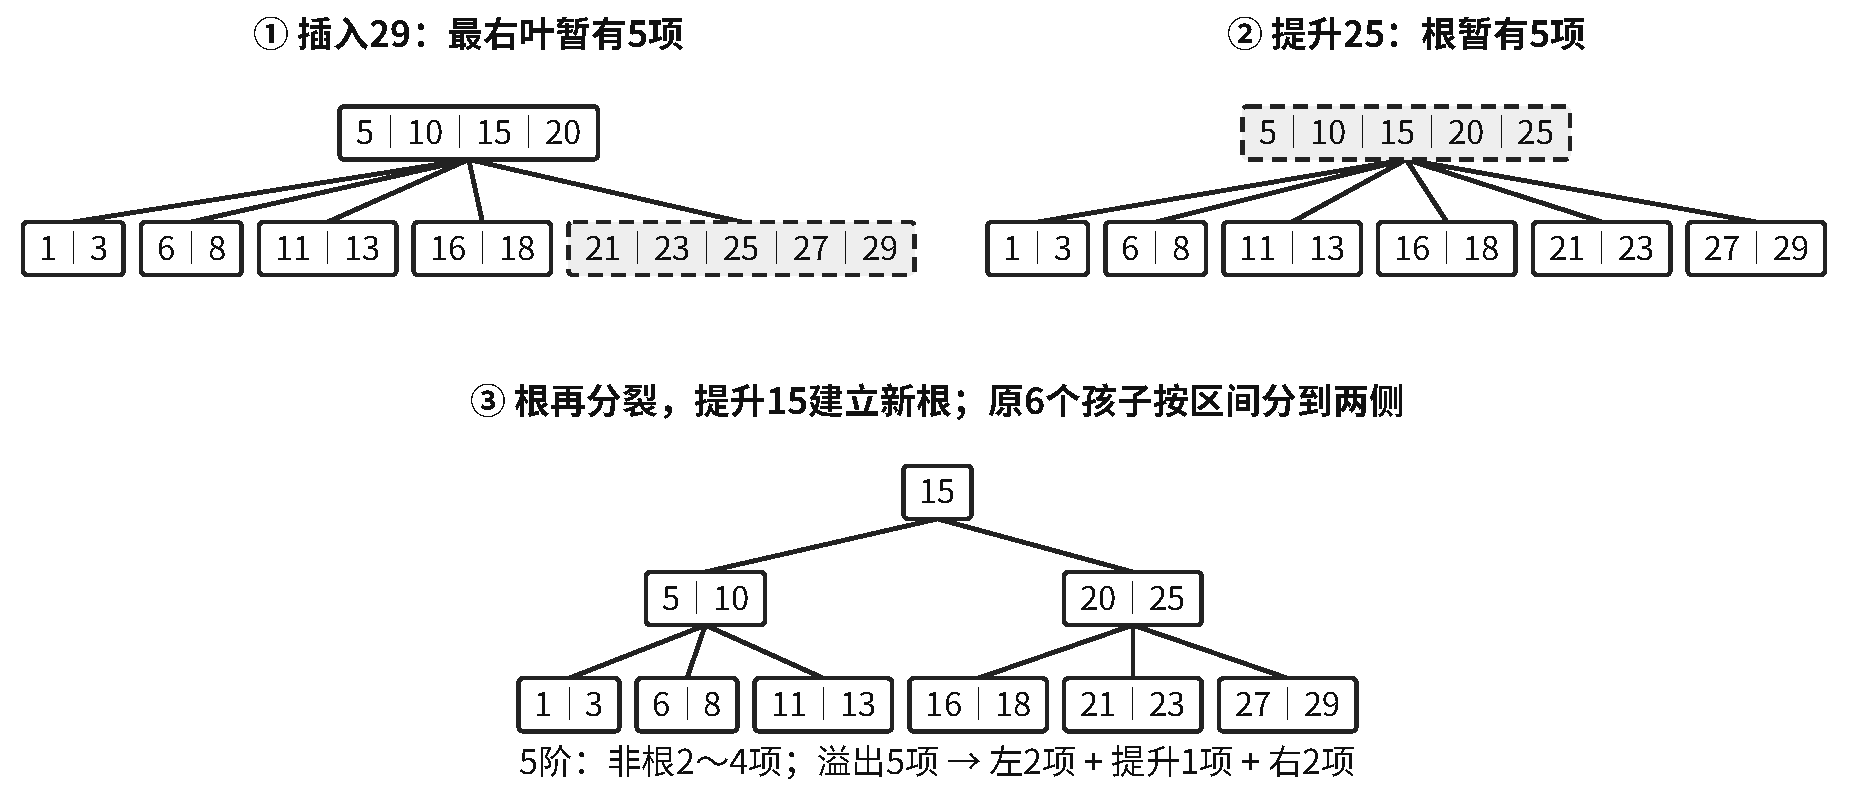
\includegraphics[width=\linewidth,height=108mm,keepaspectratio]{figures/DS_15_btree_split.pdf}
\caption{5阶B树叶分裂与根分裂}\label{DS07-btree-insert-figure}
\end{figure}

\begin{figure}[H]
\centering
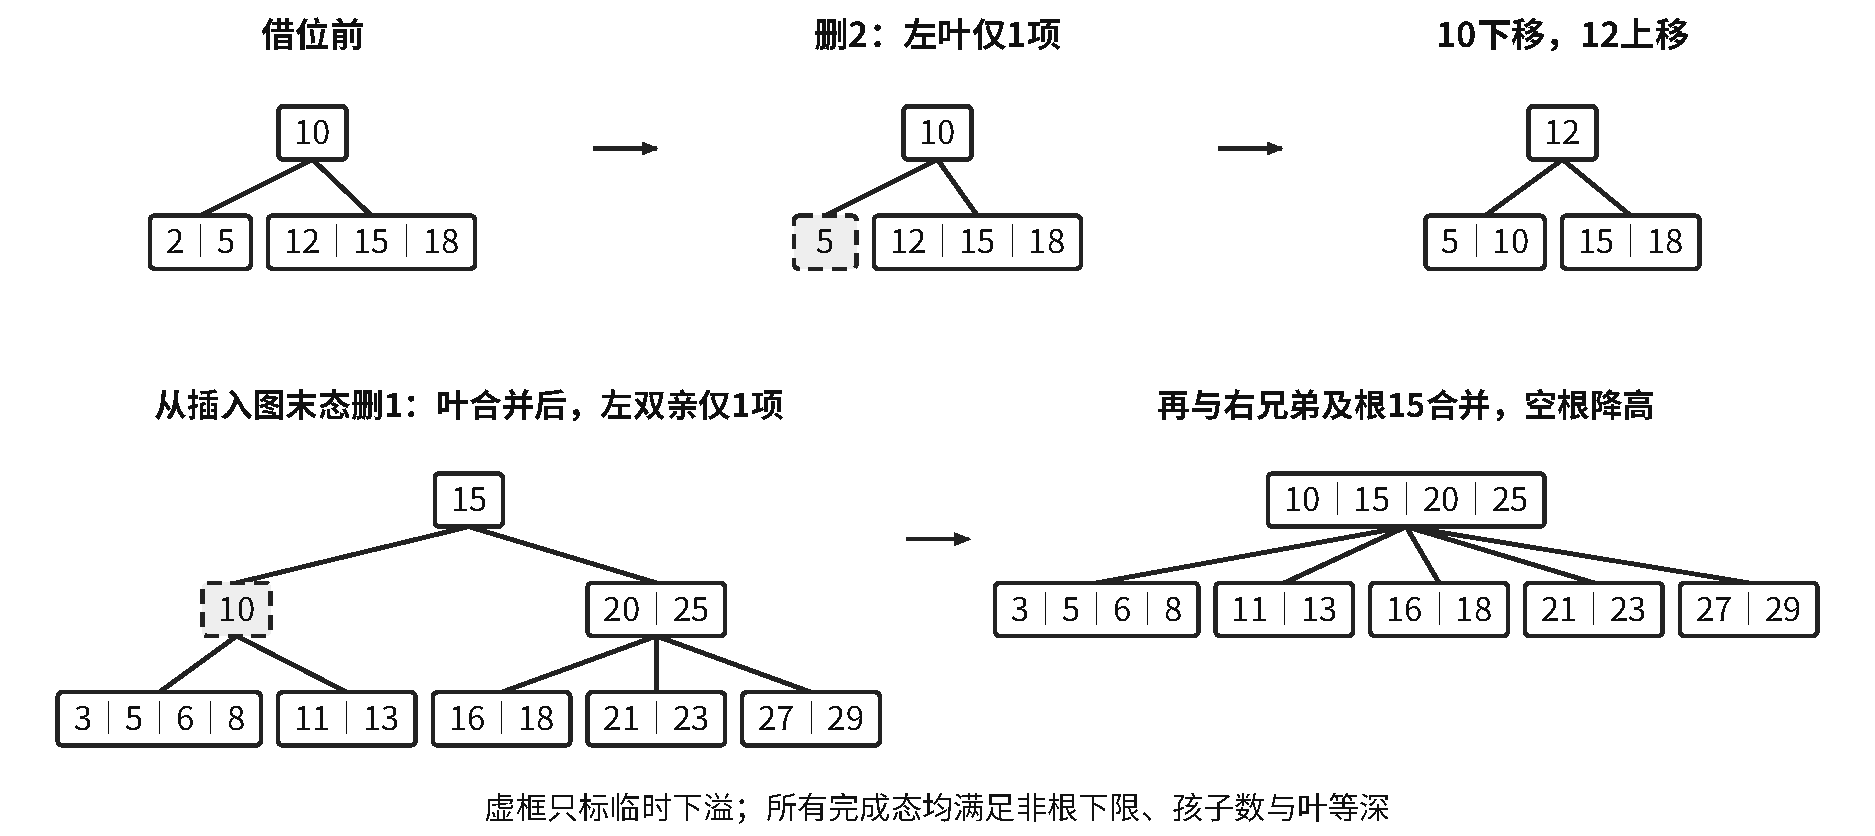
\includegraphics[width=\linewidth,height=108mm,keepaspectratio]{figures/DS_20_btree_delete.pdf}
\caption{经父分隔键借位与逐层合并}\label{DS07-btree-delete-figure}
\end{figure}

5阶每非根2至4键：两个合法2键兄弟加父键共5键，超过上限；应在删除造成一侧1键后按\(1+1+2=4\)合并。不能直接照搬其他阶数的提前合并规则。完成态须满足键有序、子树区间、容量、孩子数及底层等深。

\par\medskip\Needspace{4\baselineskip}\noindent\hypertarget{DS07-E05}{}\label{DS07-E05}\textbf{例 7-5}\par\nobreak\smallskip

一棵3阶B树共有2047个关键字，最大高度为（　），最小高度为（　）。

A. 11　B. 10　C. 8　D. 7

\par\medskip\Needspace{4\baselineskip}\noindent\hypertarget{DS07-E06}{}\label{DS07-E06}\textbf{例 7-6}\par\nobreak\smallskip

给定7个不同关键字，能构造的不同4阶B树的个数最多为（　）。

A. 7　B. 8　C. 9　D. 10

\section{B+树}\label{DS07-bplus}

记录或记录指针集中于叶层，内部层只存索引；叶含全体关键字并按序链接。点查沿根到叶，范围查先定位起点叶，再沿叶链扫描。

本章采用王道``每个内部索引键为一棵子树最大键''约定，内部键数等于孩子数：最多\(m\)，非根分支至少\(\lceil m/2\rceil\)，非叶根至少2。B树内部命中可结束，B+树记录查询仍降至叶。

\begin{figure}[H]
\centering
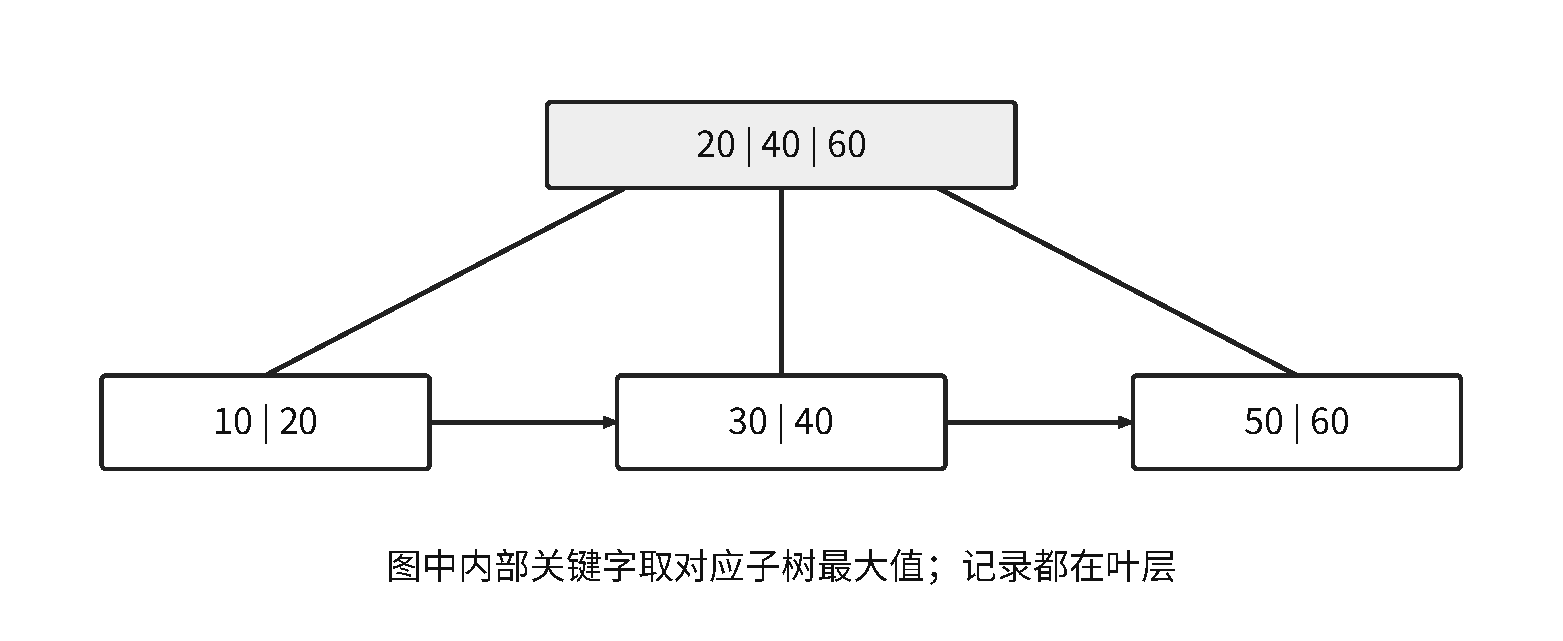
\includegraphics[width=\linewidth,height=108mm,keepaspectratio]{figures/DS_16_bplus.pdf}
\caption{B+树内部索引与有序叶链}\label{DS07-bplus-figure}
\end{figure}

每页不携整条记录通常可提高内部扇出，减少外存层数；若叶仅存记录指针，读取叶外记录的I/O另计。

\section{散列函数与冲突处理}\label{DS07-hash}

同一散列函数值的不同关键字为同义词。函数须确定、尽量均匀；装填因子\(\alpha=n/m\)，其中\(m\)为表长。

\par\smallskip
{\fontsize{9.3}{12}\selectfont\setlength{\tabcolsep}{2.5pt}\setlength{\LTleft}{0pt}\setlength{\LTright}{0pt}
\begin{longtable}{@{}>{\raggedright\arraybackslash}p{\dimexpr0.42052\linewidth-2\tabcolsep\relax}>{\raggedright\arraybackslash}p{\dimexpr0.57948\linewidth-2\tabcolsep\relax}@{}}
\toprule
构造方法 & 条件与参数 \\

\midrule\endfirsthead\toprule
构造方法 & 条件与参数 \\

\midrule\endhead\bottomrule\endfoot
直接定址\(akey+b\) & 连续且范围可控的关键字 \\

除留余数\(key\bmod p\) & \(p\)通常取不大于表长的适当素数 \\

数字分析 & 按已知分布选择均匀数位 \\

平方取中 & 让多个数位共同影响结果 \\

\end{longtable}}
\par\smallskip

开放定址统一按\(H_i=(H(key)+d_i)\bmod m\)计算，每次增量加在初始地址上；初始散列模数\(p\)与探测模数\(m\)可不同。

\par\smallskip
{\fontsize{9.3}{12}\selectfont\setlength{\tabcolsep}{2.5pt}\setlength{\LTleft}{0pt}\setlength{\LTright}{0pt}
\begin{longtable}{@{}>{\raggedright\arraybackslash}p{\dimexpr0.22944\linewidth-2\tabcolsep\relax}>{\raggedright\arraybackslash}p{\dimexpr0.32448\linewidth-2\tabcolsep\relax}>{\raggedright\arraybackslash}p{\dimexpr0.44608\linewidth-2\tabcolsep\relax}@{}}
\toprule
探测方法 & 增量 & 覆盖条件 \\

\midrule\endfirsthead\toprule
探测方法 & 增量 & 覆盖条件 \\

\midrule\endhead\bottomrule\endfoot
线性 & \(d_i=i\) & 连续\(m\)次遍历全表 \\

正平方 & \(d_i=i^2\) & 未必覆盖全表 \\

正负平方 & \(0,1,-1,4,-4,\ldots\) & \(m=4j+3\)为素数且增量充分时可覆盖 \\

双散列 & \(i\,hash_2(key)\) & 步长与\(m\)互质 \\

伪随机 & 可复现的给定增量 & 检查模\(m\)的剩余类覆盖 \\

\end{longtable}}
\par\smallskip

双散列步长必须模\(m\)非零；素数表长可用\texttt{1+\allowbreak{}(\allowbreak{}key\%(\allowbreak{}m-1)\allowbreak{})\allowbreak{}}生成合法步长，负数取模另约定。线性探测易聚集；平方探测即使表未满也可能到不了空位。

\subsection{槽状态与删除}\label{DS07-hash-state}

\par\smallskip\noindent\begin{minipage}{\linewidth}
\begin{codeblock}[language={}]
hashFind(key):
    按约定的探查序列访问地址
    若槽为有效且关键字相同: 成功
    若槽从未使用: 失败
    若槽已删除或关键字不同: 继续探查
    若可探查位置已耗尽: 失败
\end{codeblock}
\end{minipage}\par\smallskip

插入可记住首个删除槽；若禁止重复，仍须沿后续路径排除已存在同键。表满或可达探测位置耗尽时结束，防止无限循环。链地址法真实断链删除，无需墓碑。

\par\medskip\Needspace{4\baselineskip}\noindent\hypertarget{DS07-E07}{}\label{DS07-E07}\textbf{例 7-7}\par\nobreak\smallskip

长度为5、初始为空的散列表HT，\(H(k)=(k+4)\bmod5\)，线性探查处理冲突。依次插入2022、12、25，再删除25，查找失败的平均查找长度为（　）。

A. 1　B. 1.6　C. 1.8　D. 2.2

\par\medskip\Needspace{4\baselineskip}\noindent\hypertarget{DS07-E08}{}\label{DS07-E08}\textbf{例 7-8}\par\nobreak\smallskip

将20、3、11、18、9、14、7依次插入初始为空、长度11的HT。\(H(key)=(key\times3)\bmod11\)，初始地址为 \(H_0\)，冲突时 \(H_k=(H_0+k^2)\bmod11\ (k=1,2,\ldots)\)。

（1）画出HT并计算装填因子。（2）给出查找14时的关键字比较序列。（3）查找8，确认失败时的散列地址是多少？

\subsection{散列ASL的事件与分母}\label{DS07-hash-asl}

链地址成功代价为桶内比较位置，失败代价为桶长；空桶失败的关键字比较为0，空指针判断另计。若\(m\)个桶等概率失败，ASL为\(n/m\)；桶内有序链可提前失败，须重算概率与路径。

底稿序列\texttt{19,\allowbreak{}14,\allowbreak{}23,\allowbreak{}1,\allowbreak{}68,\allowbreak{}20,\allowbreak{}84,\allowbreak{}27,\allowbreak{}55,\allowbreak{}11,\allowbreak{}10,\allowbreak{}79}以\(key\bmod13\)头插入桶，非空链为\texttt{1:\allowbreak{}79→27→1→14}、\texttt{3:\allowbreak{}55→68}、\texttt{6:\allowbreak{}84→19}、\texttt{7:\allowbreak{}20}、\texttt{10:\allowbreak{}10→23}、\texttt{11:\allowbreak{}11}。成功ASL为\(21/12\)，13桶等概率失败ASL为\(12/13\)。

同序列放表长16、初始\(key\bmod13\)、线性探测模16：0为空，1至12依次为\texttt{14,\allowbreak{}1,\allowbreak{}68,\allowbreak{}27,\allowbreak{}55,\allowbreak{}19,\allowbreak{}20,\allowbreak{}84,\allowbreak{}79,\allowbreak{}23,\allowbreak{}11,\allowbreak{}10}，13至15为空。成功ASL为\(30/12=2.5\)。失败初始地址只有0至12，探测长度\texttt{1,\allowbreak{}13,\allowbreak{}12,\allowbreak{}11,\allowbreak{}10,\allowbreak{}9,\allowbreak{}8,\allowbreak{}7,\allowbreak{}6,\allowbreak{}5,\allowbreak{}4,\allowbreak{}3,\allowbreak{}2}，故失败ASL为\(91/13=7\)。删除20留标记后，成功ASL为\(29/11\)，失败ASL仍为7。

\section{按操作约束选择查找结构}\label{DS07-comparison}

\par\smallskip
{\fontsize{9.3}{12}\selectfont\setlength{\tabcolsep}{2.5pt}\setlength{\LTleft}{0pt}\setlength{\LTright}{0pt}
\begin{longtable}{@{}>{\raggedright\arraybackslash}p{\dimexpr0.22841\linewidth-2\tabcolsep\relax}>{\raggedright\arraybackslash}p{\dimexpr0.33667\linewidth-2\tabcolsep\relax}>{\raggedright\arraybackslash}p{\dimexpr0.43493\linewidth-2\tabcolsep\relax}@{}}
\toprule
结构 & 查找代价 & 适用条件与维护 \\

\midrule\endfirsthead\toprule
结构 & 查找代价 & 适用条件与维护 \\

\midrule\endhead\bottomrule\endfoot
顺序查找 & 最坏\(O(n)\) & 可无序，无有序维护 \\

折半 & \(O(\log n)\) & 有序顺序表，插删移动最坏\(O(n)\) \\

普通BST & \(O(h)\)，最坏\(O(n)\) & 动态、有序，可能退化 \\

AVL、红黑树 & 最坏\(O(\log n)\) & 动态更新并维护平衡性质 \\

B、B+树 & 至多\(h\)次索引页读取 & 多路外存索引；B+适合叶链范围访问 \\

散列 & 合适函数与负载下平均\(O(1)\) & 等值检索；链法最坏\(O(n)\)，开放定址最坏\(O(m)\) \\

\end{longtable}}
\par\smallskip

有序范围检索需要关键字次序；散列扩容、树旋转、索引更新均属于维护代价。
